    \documentclass[12pt,final,fleqn]{article}

% basic packages
\usepackage[margin=1in] { geometry }
\usepackage{amssymb,amsmath, bm}
\usepackage{verbatim}
\usepackage[latin1]{inputenc}
%\usepackage[OT1]{fontenc}
\usepackage{setspace}
\usepackage{enumitem}
\usepackage[bottom]{footmisc}
\usepackage{url}
\usepackage[font={bf}]{caption}
\usepackage{float}
%\usepackage{pgfplots}
%\usepackage[font={bf}]{caption}
\usepackage{setspace}
\usepackage{latexsym}
%\usepackage{euscript}
\usepackage{graphicx}
\usepackage{marvosym}
\usepackage{amsmath} 
\usepackage{authblk}
\usepackage{xcolor}
\usepackage{blindtext}
%\usepackage[varg]{txfonts}  Older version of ``g'' in math.

% bibliography packages
\usepackage[natbibapa]{apacite}
\bibliographystyle{apacite}
\bibpunct{(}{)}{;}{a}{}{,}
\renewcommand{\bibname}{References}
\defcitealias{lokniti2014}{CSDS 2014}

% hyperref options
\usepackage{color}
\usepackage{hyperref}
\usepackage{xcolor}
\hypersetup{
    colorlinks,
    linkcolor={blue!50!black},
    citecolor={blue!50!black},
    urlcolor={blue!80!black}
}
\newcommand*{\Appendixautorefname}{Appendix}
\renewcommand*{\sectionautorefname}{Section}
\renewcommand*{\subsectionautorefname}{Section}
\newcommand{\aref}[1]{\hyperref[#1]{Appendix~\ref{#1}}}

% packages for tables
\usepackage{longtable}
\usepackage{booktabs, threeparttable}
\usepackage{threeparttablex}
%\usepackage{tabularx}
% dcolumn package
\usepackage{dcolumn}
\newcolumntype{.}{D{.}{.}{-1}}
\newcolumntype{d}[1]{D{.}{.}{#1}}
\captionsetup{belowskip=10pt,aboveskip=-5pt}
\usepackage{multirow}
% rotating package
\usepackage[figuresright]{rotating}
\usepackage{pdflscape}
\usepackage{subcaption}

% packages for figures
\usepackage{grffile}
\usepackage{afterpage}
\usepackage{float}
\usepackage[section]{placeins}


% theorem package
\usepackage{theorem}
\theoremstyle{plain}
\theoremheaderfont{\scshape}
\newtheorem{theorem}{Theorem}
\newtheorem{algorithm}{Algorithm}
\newtheorem{assumption}{Assumption}
\newtheorem{lemma}{Lemma}
\newtheorem{proposition}{Proposition}
\newtheorem{remark}{Remark}
\newcommand{\qed}{\hfill \ensuremath{\Box}}
\newcommand\indep{\protect\mathpalette{\protect\independenT}{\perp}}
\DeclareMathOperator{\sgn}{sgn}
\DeclareMathOperator{\tr}{tr}
\DeclareMathOperator{\argmin}{arg\min}
\DeclareMathOperator{\argmax}{arg\max}
\def\independenT#1#2{\mathrel{\rlap{$#1#2$}\mkern2mu{#1#2}}}
\providecommand{\norm}[1]{\lVert#1\rVert}
\renewcommand\r{\right}
\renewcommand\l{\left}
\newcommand\E{\mathbb{E}}
\newcommand\dist{\buildrel\rm d\over\sim}
\newcommand\iid{\stackrel{\rm i.i.d.}{\sim}}
\newcommand\ind{\stackrel{\rm indep.}{\sim}}
\newcommand\cov{{\rm Cov}}
\newcommand\var{{\rm Var}}
\newcommand\SD{{\rm SD}}
\newcommand\bone{\mathbf{1}}
\newcommand\bzero{\mathbf{0}}

% dotted lines in tables
%\usepackage{arydshln}

\usepackage{pdflscape}

% spacing between sections and subsections
\usepackage[compact]{titlesec}

% times new roman
%\usepackage{times}

% appendix settings
\usepackage[toc,page,header]{appendix}
\renewcommand{\appendixpagename}{\centering Appendices}
\usepackage{chngcntr}
\usepackage{etoolbox}
\usepackage{lipsum}


% file paths and definitions
\makeatletter
\newcommand*\ExpandableInput[1]{\@@input#1 }
\makeatother

\setlength{\mathindent}{1cm}
\allowdisplaybreaks[4]
\doublespacing
%\special{pdf: pagesize width 8.5truein height 11.0truein}

\titleformat{\subsection}
  {\itshape\large}{\thesubsection}{1em}{}

\setcounter{tocdepth}{1}

%--------------------------------------------------------------------------------------
% BEGIN DOCUMENT
%--------------------------------------------------------------------------------------

\begin{document}
\singlespace
\title{\textbf{Corruption information and vote share: A meta-analysis and lessons for survey experiments}\vspace{-1ex}\thanks{}}
%I would like to thank Peter Aronow, Alexander Coppock, Ang�le Delevoye, Devin Incerti, Joshua Kalla, Daniel Mattingly, Susan Rose-Ackerman, Frances Rosenbluth, Radha Sarkar, and Fredrik S�vje for exceptionally helpful feedback and suggestions. Any and all errors are my own.

\author{Trevor Incerti\thanks{PhD Student in the Department of Political Science, Yale University. trevor.incerti@yale.edu}\vspace{-2ex}}
%\affil{\textit{Yale University}\vspace{-2.5ex}}
%\date{\today}
\date{\today}
\maketitle

\begin{abstract}
\noindent
Do voters hold politicians accountable for corruption? Field experiments that provide voters with information about corrupt acts of politicians then monitor vote choice are now standard. Similarly, vote-choice survey experiments commonly inform respondents of corrupt acts of hypothetical candidates. What have we learned from these experiments? Meta-analysis demonstrates that the aggregate treatment effect of corruption information on vote share in field experiments is approximately zero. By contrast, corrupt candidates are punished by approximately 33-35 percentage points across survey experiments. This suggests that while vote-choice survey experiments may identify the effect of informational treatments in hypothetical scenarios, the point estimates they provide may not be representative of real-world voting behavior. I explore publication bias, social desirability bias, and the nature of the experimental designs as potential explanations for this discrepancy. Finally, I offer suggestions for analyzing vote-choice conjoint experiments when researchers have strong theories about the conditions that shape voter decision-making.
\end{abstract}

\doublespace

\begin{center}
\textcolor{red}{[PRELIMINARY DRAFT: ADDITIONAL STUDIES TO BE ADDED AND POINT ESTIMATES REFINED. PLEASE DO NOT CITE OR CIRCULATE WITHOUT AUTHOR'S PERMISSION.]}
\end{center}

\pagebreak

\section{Introduction} \label{sec:Introduction}

Competitive elections create a system whereby voters can hold policy makers accountable for their actions. This mechanism should make politicians hesitant to engage in malfeasance such as blatant acts of corruption. Increases in public information regarding corruption should therefore decrease levels of corruption in government, as voters armed with information should expel corrupt politicians \citep{gray1998corruption, kolstad2009transparency, rose2016corruption}. However, this theoretical prediction is undermined by the observation that well-informed voters continue to vote corrupt politicians into office in many democratic states. Political scientists and economists have therefore turned to experimental methods to test the causal effect of learning about politician corruption on vote choice.

Numerous experiments have examined whether providing voters with information about the corrupt acts of politicians decreases their re-election rates. These papers  often suggest that there is little consensus on how voters respond to information about corrupt politicians \citep{botero2015says, buntaine2018sms, arias2018priors, klavsnja2017voters, solaz2018group, de2017electoral}. Others indicate that experiments have provided us with evidence that voters strongly punish individual politicians involved in malfeasance \citep{chong2014does, winters2015political, winters2016s, weitz2017can}.

By contrast, this meta-analysis suggests that: (1) In aggregate, the effect of providing information about incumbent corruption on incumbent vote share in field experiments is approximately zero, and (2) corrupt candidates are punished by respondents by approximately 33-35 percentage points across survey experiments. I also examine mechanisms that may give rise to this discrepancy. I do not find systematic evidence of publication bias. Social desirability bias may lead survey experiments to capture anti-corruption norms rather than realistic voter behavior. Field and survey experiments also may be measuring different causal estimands due to contextual differences. Conjoint experiments attempt to alleviate some of these issues, but are often analyzed in ways that may fail to illuminate the most substantively important comparisons.  


\section{Corruption information and electoral accountability} \label{sec: information}

Experimental support for the hypothesis that providing voters with information about politicians' corrupt acts decreases their re-election rates is mixed. Field experiments have provided some causal evidence that informing voters of candidate corruption has negative (but generally small) effects on candidate vote-share. This information has been provided by: randomized financial audits \citep{ferraz2008exposing}, fliers revealing corrupt actions of politicians \citep{de2011voters, chong2014does}, and SMS messages \citep{buntaine2018sms}. However, near-zero and null findings are also prevalent, and the negative and significant effects reported above sometimes only manifest in particular subgroups. \citet{banerjee2010can} primed voters in rural India not to vote for corrupt candidates, and \citet{banerjee2011informed} provided information on politicians' spending discrepancies, with both studies finding near-zero and null effects on vote share. \citet{boas2018norms} similarly find zero and null effects from distributing fliers in Brazil. Finally, \citet{arias2018priors, arias2019information} find that providing Mexican voters with information (fliers) about mayoral corruption actually \textit{increased} incumbent party vote share by 3\%.\footnote{The authors theorize that this average effect stems from levels of reported malfeasance actually being lower than voters no-information expectations of corruption.} 

By contrast, online survey experiments consistently show large negative effects from information treatments on hypothetical vote share. These experiments often manipulate moderating factors other than information provision (e.g. quality of information, source of information, whether the candidate is a co-partisan or co-ethnic, whether corruption brings economic benefits, etc.), but even so systematically show negative treatment effects \citep{avenburg2016corruption, anduiza2013turning, banerjee2014poor, breitenstein2019choosing, boas2018norms, eggers2018corruption, franchino2015voting, klavsnja2013economy, klavsnja2017voters, mares2019voting, vera2017heterogeneous, winters2013lacking, winters2015political, winters2016s, weitz2017can, winters2018information}. These experiments have historically taken the form of single treatment arm or multiple arm factorial vignettes, but more recently have tended toward conjoint experiments \citep{mares2019voting, klavsnja2017voters, franchino2015voting, breitenstein2019choosing, chauchard2017limited}.

\citet{boas2018norms} find differential results in a pair of matched field and survey experiments conducted in Brazil---zero and null in field, large and negative in survey. They argue that this may reflect that norms against malfeasance in Brazil do not translate into action in real life. \citet{boas2018norms} point to features specific to Brazil in their explanation of this discrepancy, namely lower salience of corruption to Brazilian voters in municipal elections and the strong effects of dynastic politics. However, meta-analysis demonstrates that this is not only the case for \citet{boas2018norms}'s experiments in Brazil, but extends across a systematic review of all studies conducted to date. This suggests that the discrepancy between field and survey experimental findings is driven by methodological differences, rather than features specific to Brazilian voters. 

Lab experiments that reveal corrupt actions to fellow players appear to be similar to survey experiments, and also show large negative treatment effects (see \autoref{fig: lab}). While there are not enough lab experiments examining whether the provision of corruption information impacts vote choice to conduct a formal meta-analysis \citep{arvate2017condemning, azfar2007transparency, solaz2018group, rundquist1977corrupt}, this discrepancy is worth noting as previous examinations of lab-field correspondence have found evidence of general replicability \citep{camerer2011promise, coppock2015assessing}.

\section{Research Design and Methods} \label{sec: Methods}

\subsection{Selection criteria}\label{sec: criteria}

I followed standard practices to locate the experiments included in the meta-analysis. This included following citation chains and searches of data bases using the terms (``corruption experiment,'' ``corruption field experiment,'' ``corruption survey experiment,'' ``corruption factorial'', ``corruption candidate choice'', ``corruption conjoint'', ``corruption, vote, experiment'', and ``corruption vignette''). Papers from any discipline are eligible for inclusion, but in practice stem only from economics and political science. Both published articles and working papers are included so as to ensure the meta-analysis is not biased towards published results. In total, I located 10 field experiments from 8 papers, and 18 survey experiments from 15 papers.

Field experiments are included if researchers randomly assigned information regarding incumbent corruption to voters, then measured corresponding voting outcomes. This therefore excludes experiments that randomly assign corruption information, but use favorability ratings or other metrics rather than actual vote share as their dependent variable. I include one natural experiment, \citet{ferraz2008exposing}, as random assignment was conducted by the Brazilian government. Effects reported in the meta-analysis come from information treatments on the entire sample of study only, not subgroup or interactive effects that reveal the largest treatment effects.

For survey experiments, studies must test a no-information control group versus a corruption information treatment group and measure vote choice for a hypothetical candidate. This necessarily excludes studies that compare one type of information provision (e.g. source) to another and the control group is one type of information rather than no information, or where the politician is always known to be corrupt \citep{konstantinidis2013sources, botero2015says, anduiza2013turning, rundquist1977corrupt, munoz2012voters, weschle2016punishing}. In many cases, studies have multiple corruption treatments (e.g. high quality information vs. low quality information, co-partisan vs. opposition party, etc.). In these cases, I replicate the studies and code corruption as a binary treatment (0 = clean, 1 = corrupt) where \textit{all} treatment arms that provide corruption information are combined into a single treatment. Studies that use non-binary vote choices are rescaled into a binary vote choice.\footnote{For example, a 1-4 scale is recoded so that 1 or 2 is equal to no vote, and 3 or 4 is equal to a vote.} In some cases (5 total), point estimates, standard errors and/or confidence intervals are not explicitly reported, and standard errors are estimated by digitally measuring coefficient plots.\footnote{I recognize that this introduces non-statistical measurement error into the meta-analysis. However, it is not possible for these errors to be large enough to effect the substantive conclusions of the analysis.}

\subsection{Included studies}\label{sec: included}

A list of all papers - disaggregated by field and survey experiments - that meet the criteria outlined above are provided in \autoref{tab:field} and \autoref{tab:survey}. A list of lab experiments (4 total) can also be found in and \autoref{tab:lab}, although these studies are not included in the meta-analysis. A list of excluded studies with justification for their exclusion can be found in \autoref{tab:excluded}.

\begin{table}[!htbp] \centering 
  \caption{Field experiments}
  \label{tab:field} 
  \small
\begin{tabular}{@{\extracolsep{0pt}} cccccccc} 
\\[-1.8ex]\hline 
\hline \\[-1.8ex] 
 Study & Country & Treatment \\ 
\hline \\[-1.8ex] 
\citet{arias2018priors} & Mexico & Fliers \\
\citet{banerjee2010can} & India & Newspaper \\
\citet{banerjee2011informed} & India & Canvas/Newspaper \\
\citet{boas2018norms} & Brazil & Fliers \\
\citet{buntaine2018sms} & Ghana & SMS \\
\citet{chong2014does} & Mexico & Fliers \\
\citet{de2011voters} & Brazil & Fliers \\
\citet{ferraz2008exposing} & Brazil &  Audits \\ 
%\citet{humphreys2012policing} & Uganda & Fliers \\
\hline \\[-1.8ex] 
\end{tabular} 
\end{table} 
\FloatBarrier

\begin{table}[!htb] \centering 
  \caption{Survey experiments}
  \label{tab:survey} 
  \small
\begin{tabular}{@{\extracolsep{5pt}} cccccccc} 
\\[-1.8ex]\hline 
\hline \\[-1.8ex] 
 Study & Country & Type of survey \\ 
\hline \\[-1.8ex] 
\citet{avenburg2016corruption} & Brazil & Vignette  \\
\citet{banerjee2014poor} & India & Vignette \\
\citet{breitenstein2019choosing} & Spain & Conjoint \\
\citet{boas2018norms} & Brazil & Vignette \\
\citet{chauchard2017limited} & India & Conjoint \\
\citet{eggers2018corruption} & UK & Conjoint \\
\citet{franchino2015voting} & Italy & Conjoint \\
\citet{klavsnja2013economy} & Sweden & Vignette \\
\citet{klavsnja2013economy} & Moldova & Vignette \\
\citet{klavsnja2017voters} & Argentina & Conjoint \\
\citet{klavsnja2017voters} & Chile & Conjoint \\
\citet{klavsnja2017voters} & Uruguay & Conjoint \\
\citet{mares2019voting} & Romania & Conjoint \\
\citet{vera2017heterogeneous} & Peru & Vignette \\
\citet{winters2013lacking} & Brazil & Vignette \\
\citet{winters2015political} & Brazil & Vignette \\
\citet{winters2016s} & Brazil & Vignette \\
\citet{weitz2017can} & Brazil & Vignette \\
\citet{winters2018information} & Argentina & Vignette \\
\hline \\[-1.8ex] 
\end{tabular} 
\end{table} 
\FloatBarrier

\subsection{Additional selection comments}\label{sec: additional_comments}

Additional justification for the inclusion or exclusion of certain studies, as well as coding and/or replication choices may be warranted in some cases. The field experiment conducted by \citet{banerjee2010can} is included. However, the authors treated voters with a campaign not to vote for corrupt candidates, but did not provide voters with information on which candidates were corrupt. Similarly, the field experiment conducted by \citet{banerjee2011informed} is included, but their treatment provided information on politicians' spending discrepancies, which may imply corruption but is not as direct as other types of information provision. The results are not sensitive to the inclusion of these studies (see \autoref{fig: meta-field_no_banerjee}). The point estimates remain approximately zero percentage points using random effects estimation, and are approximately -1 percentage point using fixed effects estimation. 

With respect to survey experiments, \citet{chauchard2017limited} include two treatments, wealth accumulation and whether the wealth accumulation was illegal. The effect reported here is the illegal treatment only. This is likely a conservative estimate, as the true effect is a combination of illegality and wealth accumulation. \citet{winters2016s} and \citet{weitz2017can} report results from the same survey experiment. The results are therefore only reported once. The survey experiment in \citet{de2011voters} is excluded from the analysis as it does not use hypothetical candidates, but instead asks voters if they would have changed their actual voting behavior in response to receiving corruption information. This study has a slightly positive and null finding. The overall results are not sensitive to the inclusion of this estimate (see \autoref{fig: meta-field_defig}). 

\pagebreak

\section{Results}\label{sec: results}

\begin{figure}[!htb]
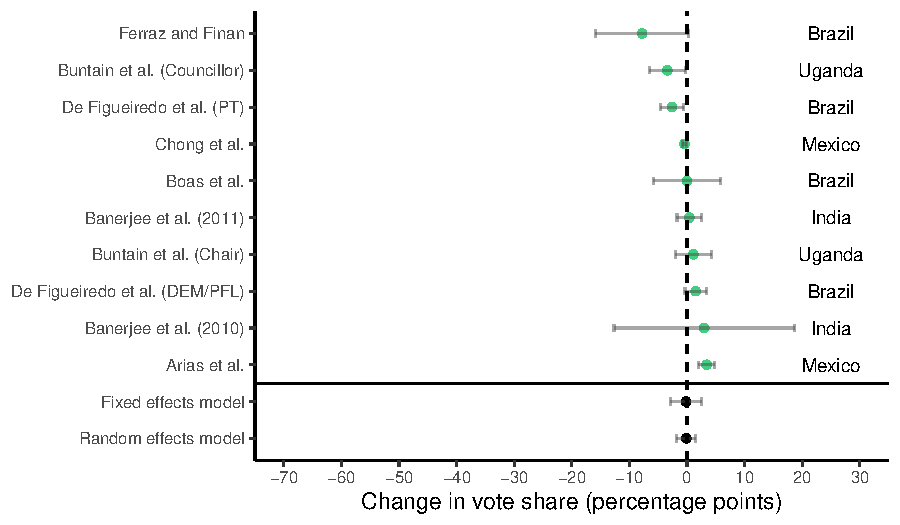
\includegraphics{../figs/field.pdf}
\vspace{0.2cm}
\caption{Field experiments: Average treatment effect of corruption information on incumbent vote share and 95\% confidence intervals}
\small
\vspace{-0.3cm}
\label{fig: meta-field}

\vspace{1.5cm}

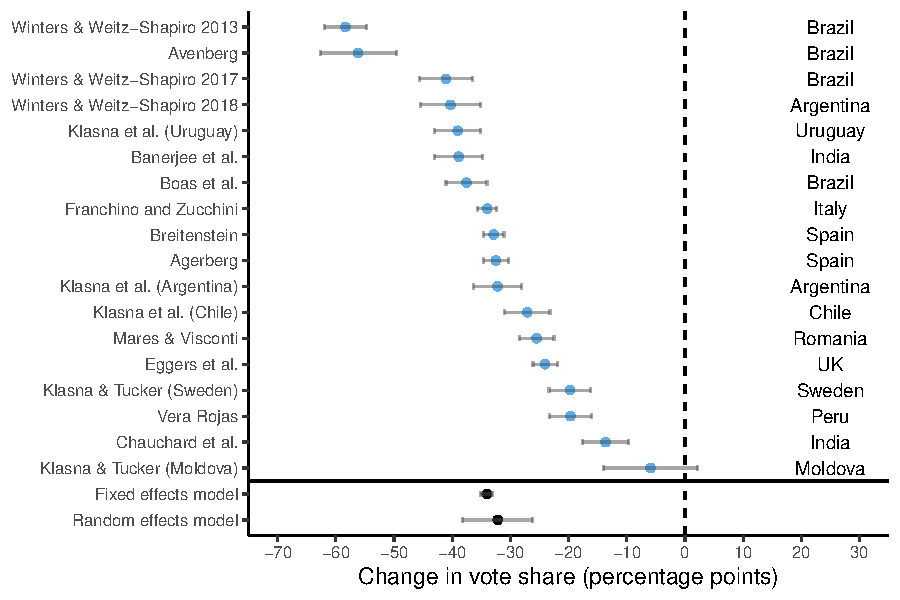
\includegraphics{../figs/survey.pdf}
\vspace{0.2cm}
\caption{Survey experiments: Average treatment effect of corruption information on incumbent vote share and 95\% confidence intervals}
\small
\vspace{-0.3cm}
\label{fig: meta-survey}
\end{figure}

Survey experiments demonstrate much larger negative treatment effects of providing information about corruption to voters relative to field experiments. In fact, the field-experimental results in \autoref{fig: meta-field} reveal a point estimate of approximately zero and suggest that we cannot reject the null hypothesis of no treatment effect.  While recognizing the power constraints inherent in such a small sample size, a univariate Shapiro-Wilk test of normality suggests that we cannot reject the null hypothesis that the point estimates are distributed normally around a mean of approximately zero percentage points. 

By contrast, corrupt candidates are punished by respondents by approximately 35 percentage points in survey experiments based on fixed effects meta-analysis and 33 percentage points using random effects meta-analysis. Of the 18 survey experiments, only one shows a null effect \citep{klavsnja2013economy}, while all others are negative and significantly different from zero at conventional levels. 

Examining all studies together, a test for heterogeneity by type of experiment (field or survey) reveals that up to 66\% of the total heterogeneity across studies can be accounted for by a dummy variable for type of experiment (0 = field, 1 = survey). This dummy variable has a significant association with the effectiveness of the information treatment at the 1\% significance level. In fact, with this dummy variable included, the overall estimate across studies is approximately 0, while the point estimate of the survey dummy is -0.32.\footnote{Using a mixed effects model with a field experiment moderator.} This implies that the predicted treatment effect across experiments is not significantly different from zero when an indicator for type of experiment is included in the model. 

\section{Exploring the discrepancy} \label{sec: discussion}

What accounts for the large difference in treatment effects between field and survey experiments? One possibility is publication bias. Null results may be less likely to be published than significant results, particularly in a survey setting. A second possibility is social desirability bias, which may cause respondents in survey experiments to report normatively desirable outcomes. Alternatively, survey settings may not mirror real-world voting decisions. Two potential ways in which the survey setting may differ from the field are: noncompliance and costliness/decision complexity. Noncompliance may decrease treatment effect sizes in field experiments. Finally, surveys may not capture the complexity and costliness of real-world voting decisions. It is possible that more complex factorial designs - such as conjoint experiments - may more successfully approximate real-world settings, and by extension field experiments. However, common methods of analysis of survey experiments may not capture all theoretical quantities of interest.

\subsection{Publication bias and p-hacking}\label{sec: publication}

Of the ten field experiments I located, only six are published. By contrast, for survey experiments only three of the 15 papers remain unpublished, and these are recent drafts. This may reflect that the null results from field experiments are less likely to be published than their survey counterparts with large and highly significant negative treatment effects, even when standard errors are relatively small. While recognizing that the sample size of studies is small, OLS and multinomial logistic regression do not indicate that reported p-value is a significant predictor of publication status, although the directionality of coefficients is consistent with lower p-values being more likely to be published. 

In order to more formally test for publication bias, I first use the p-curve developed in \citet{simonsohn2014p1, simonsohn2014p2} and \citet{simonsohn2015better}. The p-curve is based on the premise that only ``significant'' results are typically published, and depicts the distribution of statistically significant p-values for a set of published studies. The shape of the p-curve is indicative of whether or not the results of a set of studies are derived from true effects, or from publication bias. If effect sizes are clustered around 0.05 (i.e. the p-curve is ``left skewed''), this may be evidence of p-hacking, indicating that studies with p-values just below 0.05 are ``selectively reported.'' If the p-curve is ``right skewed'' and there are more low p-values (0.01), this is evidence of true effects. All significant survey experimental results included in the meta-analysis are significant at the 1\% level (making construction of a ``curve'' with bins of width 0.01 impossible), implying that publication bias likely does not explain the large negative treatment effects in survey experiments.\footnote{There is also no indication of publication bias at the 1\% level using this method.} For field experiments, there is not a large enough number of published experiments to make the p-curve viable. Only six studies are published, and of these only four are significant at at least the 5\% level.

Next, I test for publication bias by examining funnel plot asymmetry. A funnel plot depicts the outcomes from each study on the x-axis and their corresponding standard errors on the y-axis. The chart is overlaid with an inverted triangular confidence interval region (i.e. the ``funnel"), which should contain 95\% of the studies if there is no bias or between study heterogeneity. If studies with insignificant results remain unpublished the funnel plot may be asymmetric. Both visual inspection and regression tests of funnel plot asymmetry reveal an asymmetric funnel plot when survey and field experiments are grouped together (see \autoref{fig: funnel_re_all} and \autoref{tab: funnel}). However, this asymmetry disappears when accounting for heterogeneity by type of experiment, either with the inclusion of a field experiment moderator (dummy) variable or by analyzing field and survey experiments separately (see \autoref{fig: funnel_all_mod}, \autoref{fig: funnel_re_field}, \autoref{fig: funnel_re_survey}, and \autoref{tab: funnel}). 

In sum, while publication bias cannot be ruled out completely---particularly with such a small sample size of field experiments---there is no smoking gun. This implies that differences in experimental design likely account for the difference in the magnitude of treatment effects in field versus survey experiments, rather than publication bias.


\subsection{Social desirability bias}\label{sec: sdb}

A second possible explanation is social desirability bias, in which survey respondents under-report behavior that they believe to be socially undesirable. The respondent may perceive a particular response to be normatively desirable by society as whole, by the researcher(s) conducting the experiment, or both, and respond to the survey in accordance with that norm. In the case of corruption, respondents are likely to perceive corruption as both normatively ``wrong,'' as well as harmful to society, the economy, and their own personal well-being. They may therefore be more likely to choose the socially desirable option (no corruption), particularly when the respondent is aware that he or she is being observed by a researcher. 

The effect of social desirability bias may be stronger in a survey experiment where there are few downsides to selecting the socially desirable option. A hypothetical vignette has virtually no costs to selecting the socially desirable option, even when moderating variables are included. In a field experiment the cost of changing one's vote may be higher. Voters may have pre-existing opinions of real candidates that make them discount corruption information, or have strong material and/or ideological incentives to stick with their candidate. 

How might we overcome social desirability bias in survey experiments? One option is to eschew hypothetical candidates in favor of real candidates in experiments conducted during the timing of actual elections. Of course, for ethical reasons this limits researchers to having actual information regarding the corrupt actions of candidates. A second option is the use of list experiments or experiments which ask about the expected behavior of other individuals in response to new information. List experiments are surprisingly uncommon in corruption experiments (none of the survey experiments included here use this method), but a vote buying experiment in Nicaragua estimated that only 2\% of respondents admitted directly to being offered compensation in exchange for their vote, but 24\% of respondents admitted to the practice in a list experiment \citep{gonzalez2012vote}.  More complex factorial designs such as conjoint experiments have also been claimed to reduce social desirability bias \citep{hainmueller2014causal}. \\

\noindent
[Test hypothetical vs. real with survey experiment?] \\

\subsection{Do surveys mirror real-world voting decisions?}\label{sec: conjoint}

Contextual differences between survey and field experiments may also offer fundamentally different choice sets to voters, altering respondents' potential outcomes and thus capturing different estimands. Some possible contextual differences are discussed below. 

%Next, even if subjects (voters) and treatments (information) are similar, measured outcomes may differ due to the different contexts of the experiments. For example, consider a voter's choice between two candidates in a field experiment conducted during an election. A candidate is revealed to be corrupt to voters in a treatment group, but not to voters in control. The treated voter can cast a ballot for corrupt candidate A, or candidate B, who is clean. The control voter can cast a ballot for candidate A or candidate B, and has no corruption information. Now consider a survey experiment with a vignette in which the randomized treatment is whether the corrupt actions of a politician are revealed or not. The treated voter can vote for the corrupt candidate A or not, but no challenger exists. Likewise, the control voter can vote for clean candidate A or not, but no challenger exists. Further, the option to abstain from voting does not exist in the survey setting. These differences therefore offer fundamentally different choice sets to voters, altering respondents' potential outcomes and thus capturing different estimands.

\subsubsection{Noncompliance}

Informational treatments in field experiments (fliers, newspapers, etc.) may  be weaker in part because they can be missed by segments of the treatment group. More formally, survey experiments do not have noncompliance by design and therefore the average treatment effect (ATE) is equal to the intent-to-treat (ITT) effect, whereas field experiments present ITT estimates as they are unable to identify which individuals in the treatment area actually received and internalized the informational treatment. Ideally, we would calculate the complier average causal effect (CACE)---the average treatment effect among the subset of respondents who comply with treatment---in field experiments, but we are unfortunately unable to observe compliance in any of the corruption experiments conducted to date.

A theoretical demonstration shows how noncompliance can drastically alter the ITT. The ITT is defined as $ITT = CACE \times \pi_c$ where $\pi_C$ indicates the proportion of compliers in the treatment group. When $\pi_C = 1$, $ITT = CACE = ATE$. If the ITT = -0.0048---as fixed-effects meta-analysis estimates in field experiments---but only 10\% of treated individuals ``complied'' with the treatment by reading the flier sent to them, this implies that the CACE is $\frac{-0.0048}{0.1} = -0.048$, or approximately 5 percentage points. However, as the $ITT = \pi_c \times CACE$, any noncompliance necessarily reduces the size of the ITT. Future field experiments should therefore make an effort to build measurement of noncompliance into the research design.

Relatedly, informational treatments can be more easily ignored or forgotten in a field setting---weakening their effects---compared to a survey setting where the treatment is directly presented to the respondent and they are then forced to immediately make a vote choice. \citet{kalla2018minimal} note that this mechanism manifests even in campaign contact field experiments, where contact long before election day followed by immediate measurement of outcomes appears to persuade voters, whereas there is a null effect on vote choice on election day. This phenomenon will weaken the treatment effect even amongst compliers, further reducing the ITT. 

\subsubsection{Complexity, costliness, and conjoint experiments}

Previous researchers have noted that even if voters generally find corruption distasteful, the quality of the information provided or positive candidate attributes and policies may outweigh the negative effects of corruption to voters, mitigating the effects of information provision on vote-share.\footnote{See \citet{de2017electoral} for a comprehensive overview.} These mitigating factors will naturally arise in a field setting, but may only be salient to respondents if specifically manipulated in a survey setting. 

A number of survey experiments have therefore added factors other than corruption as mitigating variables, such as information quality, policy, economic benefit, and co-partisanship. Studies have randomized the quality of corruption information\footnote{For example, accusations from an independent anti-corruption authority may be deemed more credible than those from an opposition party, and accusations may be deemed less credible than a conviction.} \citep{botero2015says, breitenstein2019choosing, mares2019voting, banerjee2014poor, weitz2017can, winters2018information}, finding that lower quality information produces smaller negative treatment effects (see \autoref{fig: quality}), but effects still remain much larger than field experiments. Policy stances in line with voter preferences have also been shown to mitigate the impact of corruption \citep{rundquist1977corrupt, franchino2015voting}. Economic benefit has been argued to act as a similar mitigating factor, with evidence suggesting that respondents are more forgiving of corruption when it benefits them personally \citep{klavsnja2017voters, winters2013lacking}. Evidence of co-partisanship as a limiting factor to corruption deterrence is mixed. \citet{anduiza2013turning} and \citet{breitenstein2019choosing} both show that co-partisanship decreases the importance of corruption to Spanish respondents in survey experiments. \citet{solaz2018group} induce in-group attachment in a lab-experiment of UK subjects, finding that in-group membership reduces sanction of ``corrupt'' participants. However, \citet{klavsnja2017voters} find relatively small effects of co-partisanship in Argentina, Chile, and Uruguay, and \citet{rundquist1977corrupt} find null effects in the US in the 1970s. \citet{konstantinidis2013sources} also find that partisanship does not moderate punishment of corruption in a survey experiment in Greece. This evidence suggests that voters punish corruption less when it is costly to do so, and that these costly factors may differ by country.  

The fact that moderating variables may dampen the salience of corruption to voters has clearly not been lost on previous researchers. However, even the inclusion of these moderators does not move point estimates close to the (approximately zero) field setting, in which numerous moderating factors may be salient to the voter. By contrast, conjoint experiments allow researchers to randomize more candidate characteristics. In addition, conjoints force respondents to pick between two candidates, better emulating the choice required in an election. Finally, conjoints may minimize social desirability bias as they reduce the probability that the respondent is aware of the researcher's primary experimental manipulation of interest (e.g. corruption).\footnote{This is explicitly mentioned by \citet{hainmueller2014causal}, who argue that conjoint experiments give respondents ``various attributes and thus [they] can often find multiple justifications for a given choice.'' Note, however, that an experiment does not necessarily need to be a conjoint design to have this feature. Conjoint experiments encourage researchers to randomize more attributes and therefore typically contain more complex hypothetical vignettes. However, the same vignette complexity could be achieved without full randomization of these attributes. } 

However, researchers have thus far tended to present the results of conjoint experiments as average marginal component effects (AMCEs), then compare the magnitude of these effect sizes. AMCEs represents the unconditional marginal effect of an attribute (e.g. corruption) averaged over all possible values of the other attributes. However, this may or may not be a measure of substantive interest to the researcher. When researchers have strong theories about the conditions that shape voter decision-making, a more appropriate method may be to calculate average marginal effects in order to present predicted probabilities of voting for a candidate under these conditions.\footnote{This method is utilized by \citet{teele2018ties} to examine the probability of voting female or male candidates holding other candidate attributes constant, and is discussed in more detail by \citet{leeper2018measuring}.} For example, in a conjoint experiment including corruption information, this might be interpreted as the probability of voting for a candidate that is both corrupt and possesses other particular feature levels (e.g. party membership and/or policy positions), marginalizing across all other features in the experiment.

To illustrate this point, I replicate the conjoint experiment conducted in Italy by \citet{franchino2015voting} and present both AMCEs and predicted probabilities. Note that I group the ``investigated for corruption'' and ``convicted of corruption'' levels into a single ``corrupt'' level in my replications. The predicted probabilities are presented as a function of corruption and two policy positions - tax policy and same sex marriage - for conservative and liberal respondents. The charts therefore show the probability of preferring a profile that has particular levels of tax policy, same sex marriage policy, and corruption, marginalizing across all other features in the experiment.\footnote{Note that the authors correctly conclude that their typical ``respondent prefers a corrupt but socially and economically progressive candidate to a clean but conservative one.'' While I therefore illustrate how predicted probabilities can be used to draw conclusions that may be masked by examination of AMCEs alone, the authors themselves do not make this mistake.} 

A casual interpretation of the traditional AMCE plot presented in \autoref{fig: fz_amce} suggests that it is very unlikely a corrupt candidate would be chosen by a respondent. By contrast, the predicted probabilities plots presented in \autoref{fig: fz_margins_right} and \autoref{fig: fz_margins_left} show that even for corrupt candidates in the conjoint, the right policy platform presented to the right respondents can garner over 50\% of the predicted hypothetical vote. In other words, respondents find it costly to abandon their policy preferences, even if it forces them to select a corrupt candidate. 

\begin{figure}[!htb]
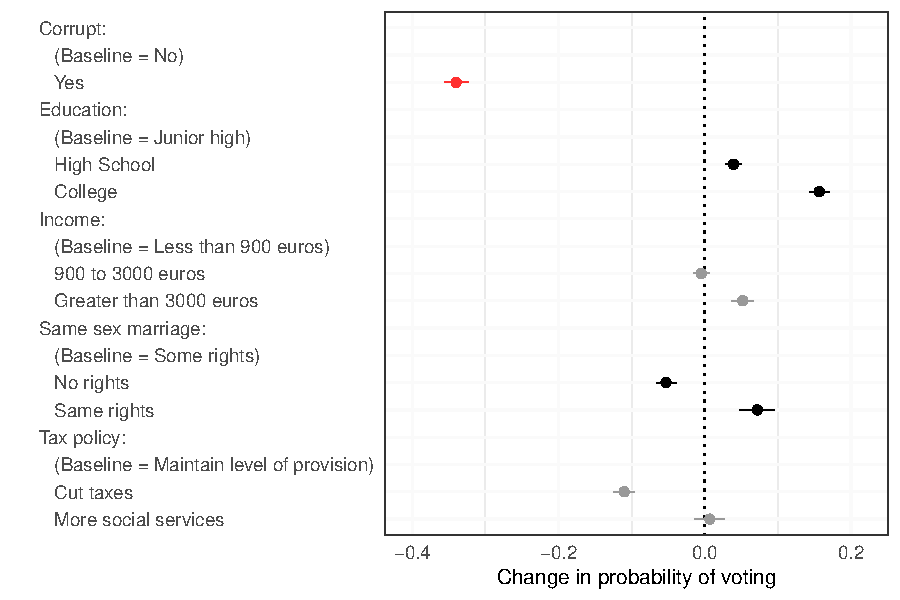
\includegraphics{../figs/fz_amce.pdf}
\caption{\citet{franchino2015voting} conjoint: average marginal component effects}
\label{fig: fz_amce}
\end{figure}


\begin{figure}[!htb]
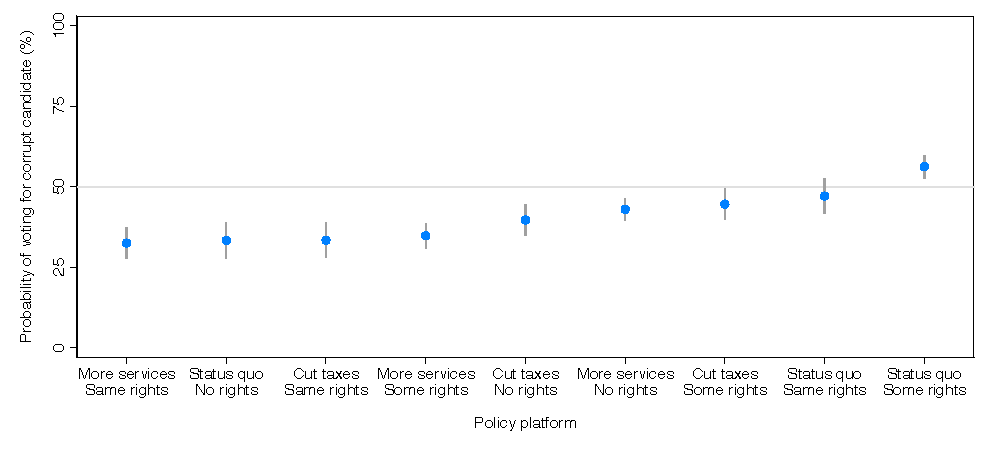
\includegraphics{../figs/fz_margins_right.pdf}
\vspace{0.2cm}
\caption{\citet{franchino2015voting} conjoint: can policy positions overcome corruption (conservative respondents)?}
\small
\vspace{-0.3cm}
\label{fig: fz_margins_right}

\vspace{1cm}

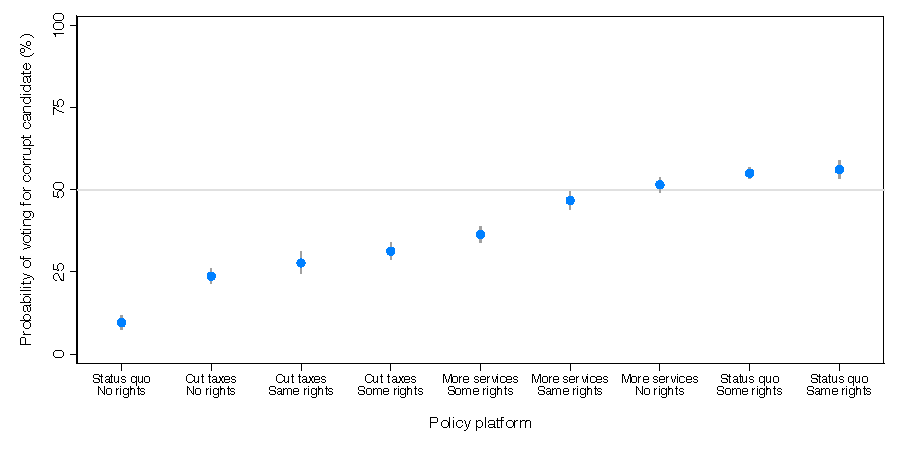
\includegraphics{../figs/fz_margins_left.pdf}
\vspace{0.2cm}
\caption{\citet{franchino2015voting} conjoint: can policy positions overcome corruption (liberal respondents)?}
\small
\vspace{-0.3cm}
\label{fig: fz_margins_left}
\end{figure}

Policy profiles that result in over 50\% of voters selecting a corrupt candidate may not be outliers in real-world scenarios. Unlike in conjoint experiments, real-world candidates' policy profiles are not selected randomly, but rather represent choices designed to appeal to voters. It may therefore be preferable to analyze conjoint experiments as above, comparing outlier characteristics (e.g. corruption) to realistic candidate profiles rather than fully randomized candidate profiles. For example, in the US context, perhaps the relevant metric of interest would be to look at the impact of corruption on vote choice for a Democratic respondent examining a Democratic candidate who espouses their preferred policy positions and attributes, rather than looking at the magnitude of the corruption AMCE versus each individual policy AMCE. \\

\noindent
[Test by comparing AMCE and ATE in survey experiments?] \\

\section{Conclusion} \label{sec: conclusion}

In an effort to test whether voters adequately hold politicians accountable for malfeasance, researchers have turned to experimental methods to measure the causal effect of learning about politician corruption on vote choice. A meta-analytic assessment of these experiments reveals that conclusions differ drastically depending on whether the experiment was deployed in the field and monitored actual vote choice, versus hypothetical vote choice in an online setting. Across field experiments, the aggregate treatment effect of providing information about corruption on vote share is approximately zero. By contrast, in survey experiments corrupt candidates are punished by respondents by approximately 33-35 percentage points. 

I explore three possible explanations that may explain this discrepancy: publication bias, social desirability bias, and contextual differences in the nature of the experimental designs. I do not find systematic evidence of publication bias. Social desirability bias may drive some of the difference if survey experiments capture anti-corruption norms rather than realistic voter behavior.  The survey setting may differ from the field due to contextual differences such as noncompliance and costliness/decision complexity. Noncompliance necessarily decreases treatment effect sizes in field experiments. High-dimension factorial designs such as conjoint experiments may better capture some of these costs in the survey setting. However, it may be preferable to analyze vote-choice conjoint experiments by comparing the probability of voting for a realistic candidate with outlier characteristics (e.g. corruption) to the probability of voting for the same realistic candidate without this characteristic, rather than examining differences in AMCEs across fully randomized candidate profiles, since these are untenable and so tell us little about real-world electoral choices. 

These findings suggest that while vote-choice survey experiments may provide information on the directionality of informational treatments in hypothetical scenarios, the point estimates they provide may not be representative of real-world voting behavior. More generally, researchers should exercise caution when interpreting actions taken in hypothetical vignettes as indicative of real world behavior such as voting. 


\clearpage
\pagebreak

\pdfbookmark[1]{References}{References}
\bibliography{bibliography}

\pagebreak

\appendix
\setcounter{table}{0}
\setcounter{figure}{0}
\renewcommand\thetable{\Alph{section}.\arabic{table}}
\renewcommand\thefigure{\Alph{section}.\arabic{figure}}
\section{Appendix} \label{Appendix}

\subsection{Lab experiments}

\begin{table}[!htbp] \centering 
  \caption{Lab experiments}
  \label{tab:lab} 
  \small
\begin{tabular}{@{\extracolsep{5pt}} cccccccc} 
\\[-1.8ex]\hline 
\hline \\[-1.8ex] 
 Study & Country & ATE \\ 
 \hline \\[-1.8ex] 
\citet{arvate2017condemning} & Brazil & Negative \\
\citet{azfar2007transparency} & USA & Negative \\
\citet{rundquist1977corrupt}\textsuperscript{1} & USA & Negative \\
\citet{solaz2018group} & UK & Negative \\
\hline \\[-1.8ex] 
\end{tabular} 
 \begin{tablenotes}
\footnotesize
\item \textsuperscript{1} The candidate is always corrupt in the \citet{rundquist1977corrupt} experiment. A ``corruption'' point estimate is therefore not provided in the coefficient plot below.
    \end{tablenotes}
\end{table} 
\FloatBarrier

\vspace{2cm}

\begin{figure}[!htb]
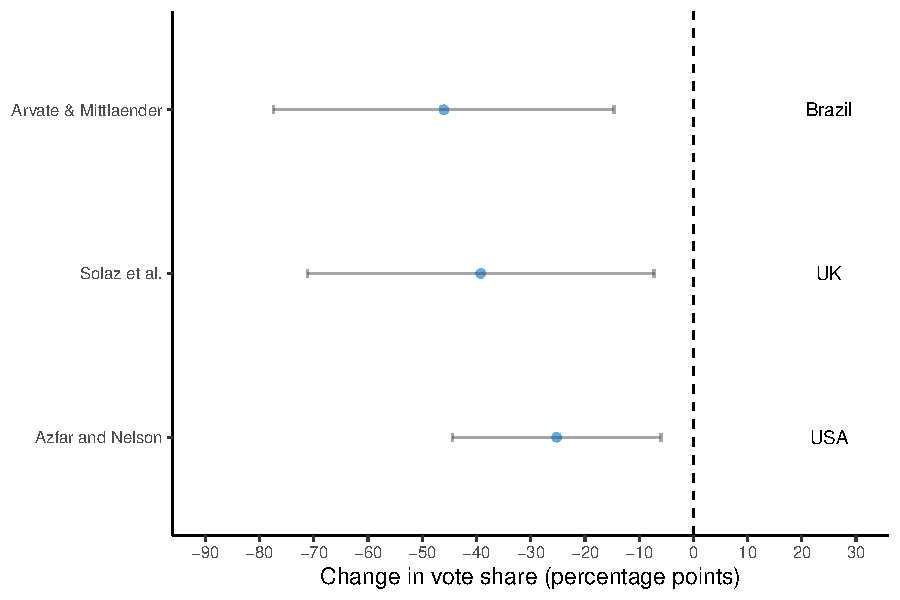
\includegraphics[scale=0.93]{../figs/lab.pdf}
\vspace{0.2cm}
\caption{Lab experiments: Average treatment effect of corruption information on vote share}.
\small
\vspace{-0.3cm}
\label{fig: lab}
\end{figure}

\pagebreak
\subsection{Excluded studies}

\begin{table}[!htbp] \centering 
  \caption{Excluded experiments}
  \label{tab:excluded} 
  \small
\begin{tabular}{@{\extracolsep{0pt}} cccccccc} 
\\[-1.8ex]\hline 
\hline \\[-1.8ex] 
 Study & Type & Reason for exclusion \\ 
\hline \\[-1.8ex] 
\citet{anduiza2013turning} & Survey & Lack of no-corruption control group \\
\citet{botero2015says} & Survey & Lack of no-corruption control group \\
\citet{de2011voters} & Survey & Outcome is hypothetically changing actual vote \\
\citet{green2018publicizing} & Field & Outcome is favorability rating, not vote share \\
\citet{konstantinidis2013sources} & Survey & Lack of no-corruption control group \\
\citet{munoz2012voters} & Survey & Lack of no-corruption control group \\
\citet{rundquist1977corrupt} & Lab & Lack of no-corruption control group \\
\citet{weitz2017can} & Survey & Data identical to \citet{winters2016s} \\
\citet{weschle2016punishing} & Survey & Lack of no-corruption control group \\
\hline \\[-1.8ex] 
\end{tabular} 
\end{table} 
\FloatBarrier

\pagebreak
\subsection{Robustness checks}

\begin{figure}[!htb]
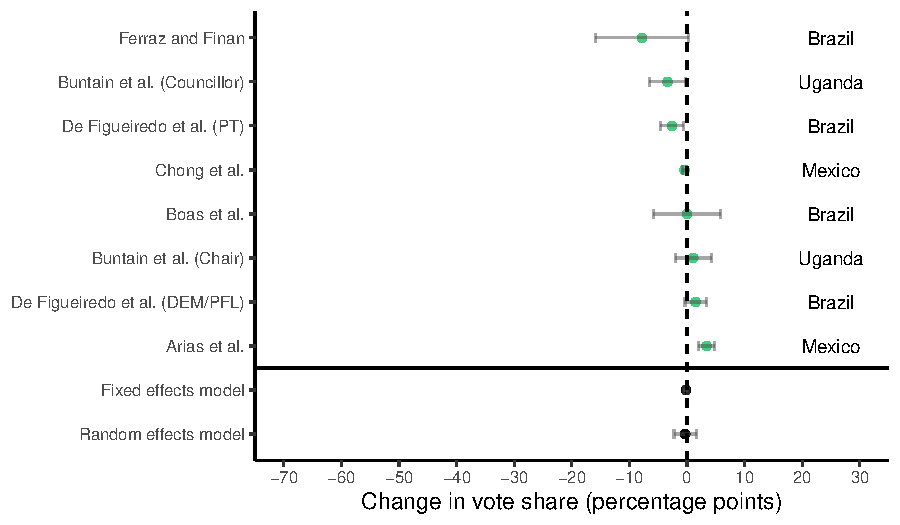
\includegraphics[scale=0.93]{../figs/field_no_banerjee.pdf}
\vspace{0.2cm}
\caption{Field experiments: Average treatment effect of corruption information on incumbent vote share (excluding \cite{banerjee2010can} and \citet{banerjee2011informed})}.
\small
\vspace{-0.3cm}
\label{fig: meta-field_no_banerjee}

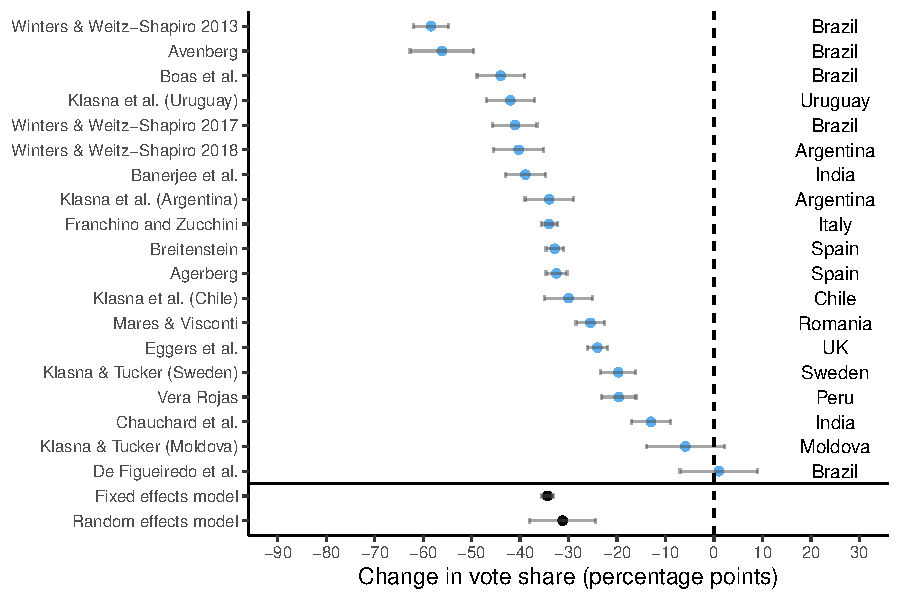
\includegraphics[scale=0.93]{../figs/survey_defig.pdf}
\vspace{0.2cm}
\caption{Survey experiments: Average treatment effect of corruption information on incumbent vote share (including \cite{de2011voters})}.
\small
\vspace{-0.3cm}
\label{fig: meta-field_defig}
\end{figure}

\pagebreak

\subsection{Publication bias}

\vspace{-.8cm}

\begin{figure}[!htb]
\begin{centering}
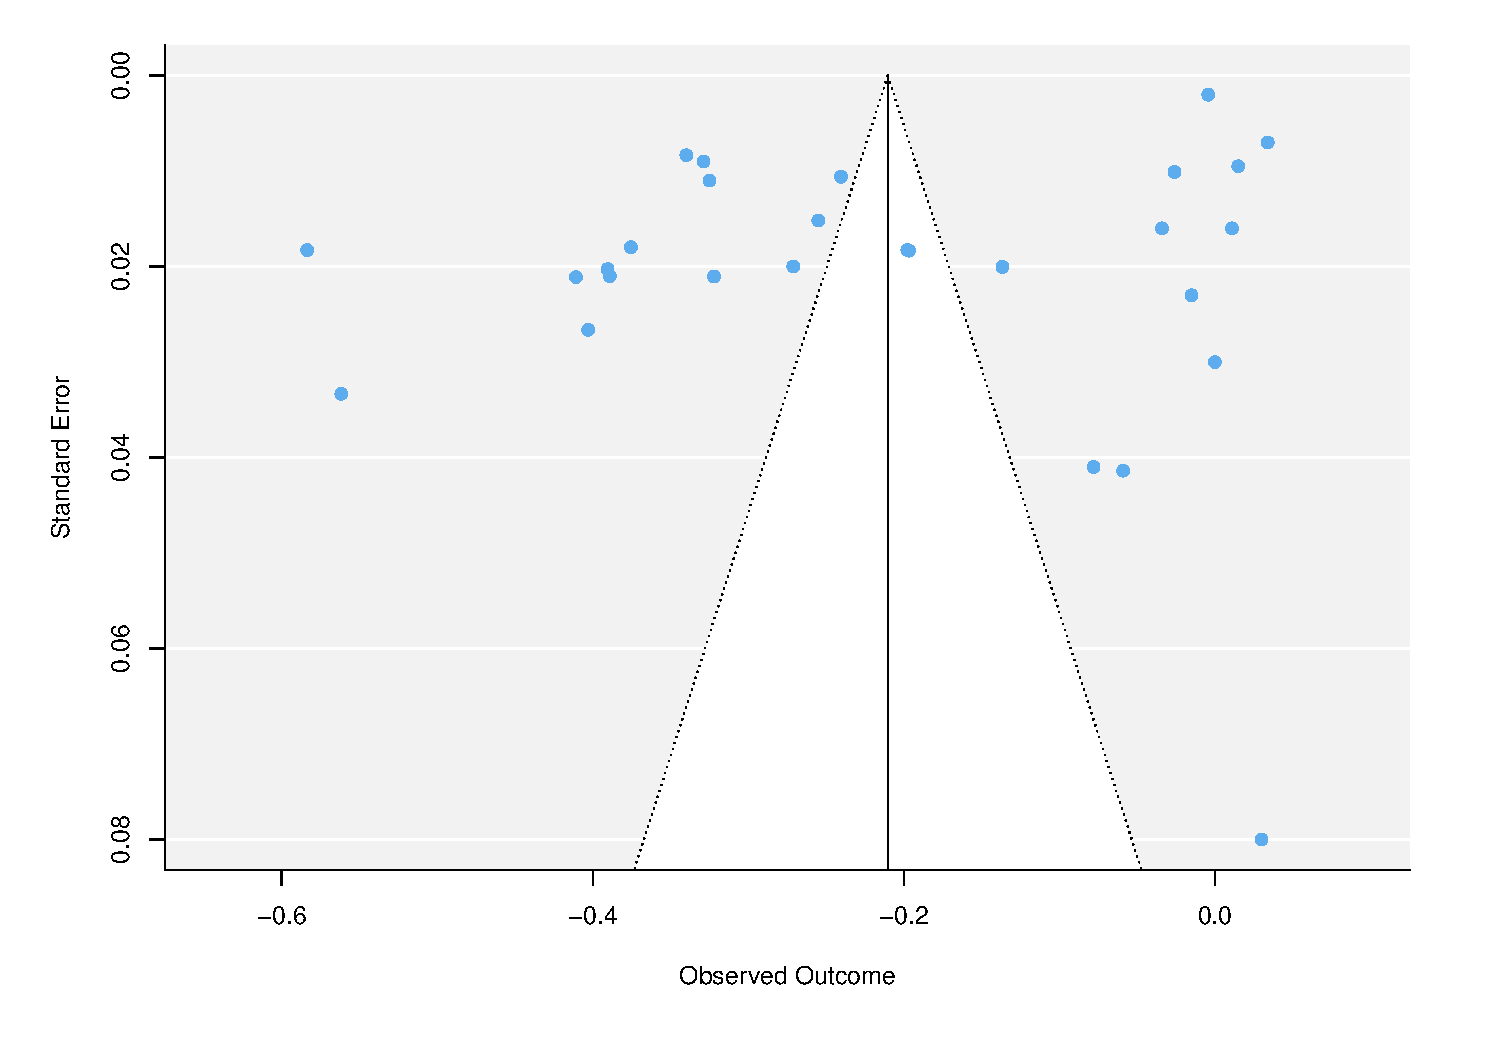
\includegraphics[scale=0.54]{../figs/funnel_re_all.pdf}
\vspace{0.2cm}
\caption{Funnel plot: all experiments}.
\small
\vspace{-0.3cm}
\label{fig: funnel_re_all}
\end{centering}
\end{figure}

\vspace{-1.3cm}

\begin{figure}[!htb]
\begin{centering}
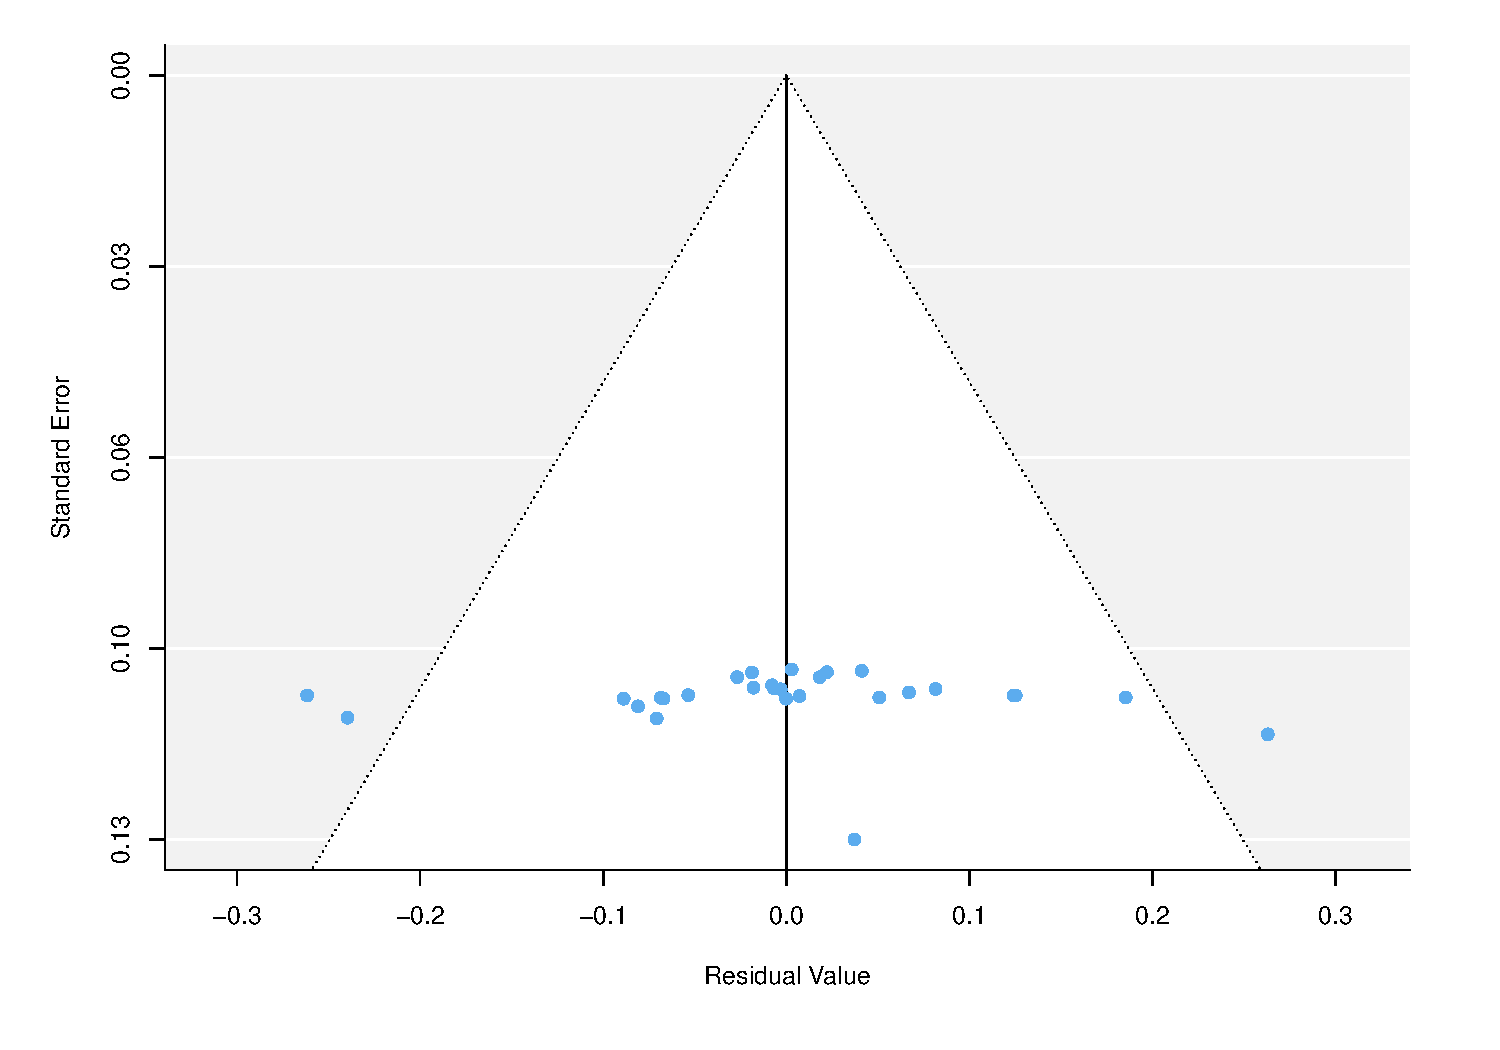
\includegraphics[scale=0.54]{../figs/funnel_all_mod.pdf}
\vspace{0.2cm}
\caption{Funnel plot: all experiments with field experiment moderator}.
\small
\vspace{-0.3cm}
\label{fig: funnel_all_mod}
\end{centering}
\end{figure}

\begin{figure}[!htb]
\begin{centering}

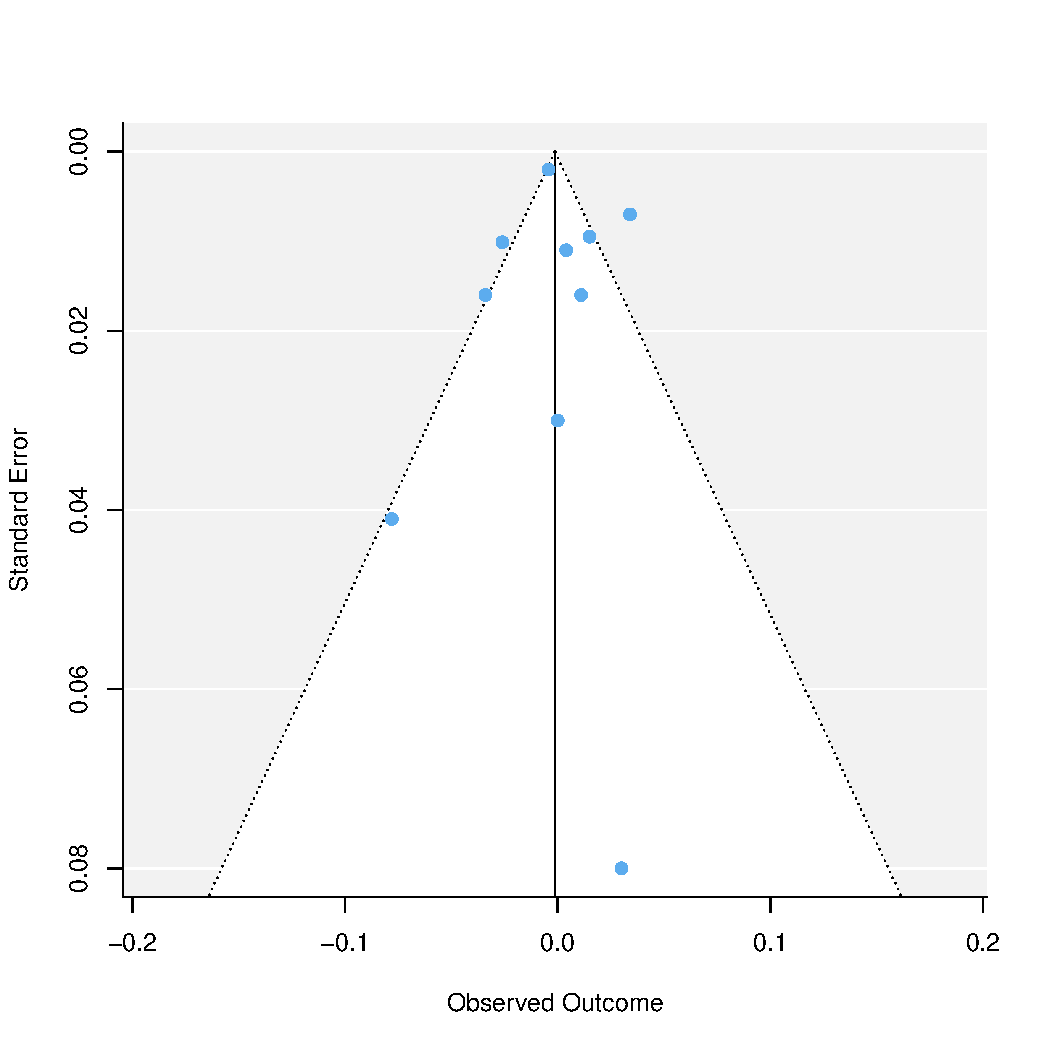
\includegraphics[scale=0.54]{../figs/funnel_re_field.pdf}
\vspace{0.2cm}
\caption{Funnel plot: field experiments}.
\small
\vspace{-0.3cm}
\label{fig: funnel_re_field}
\end{centering}
\end{figure}

\begin{figure}[!htb]
\begin{centering}
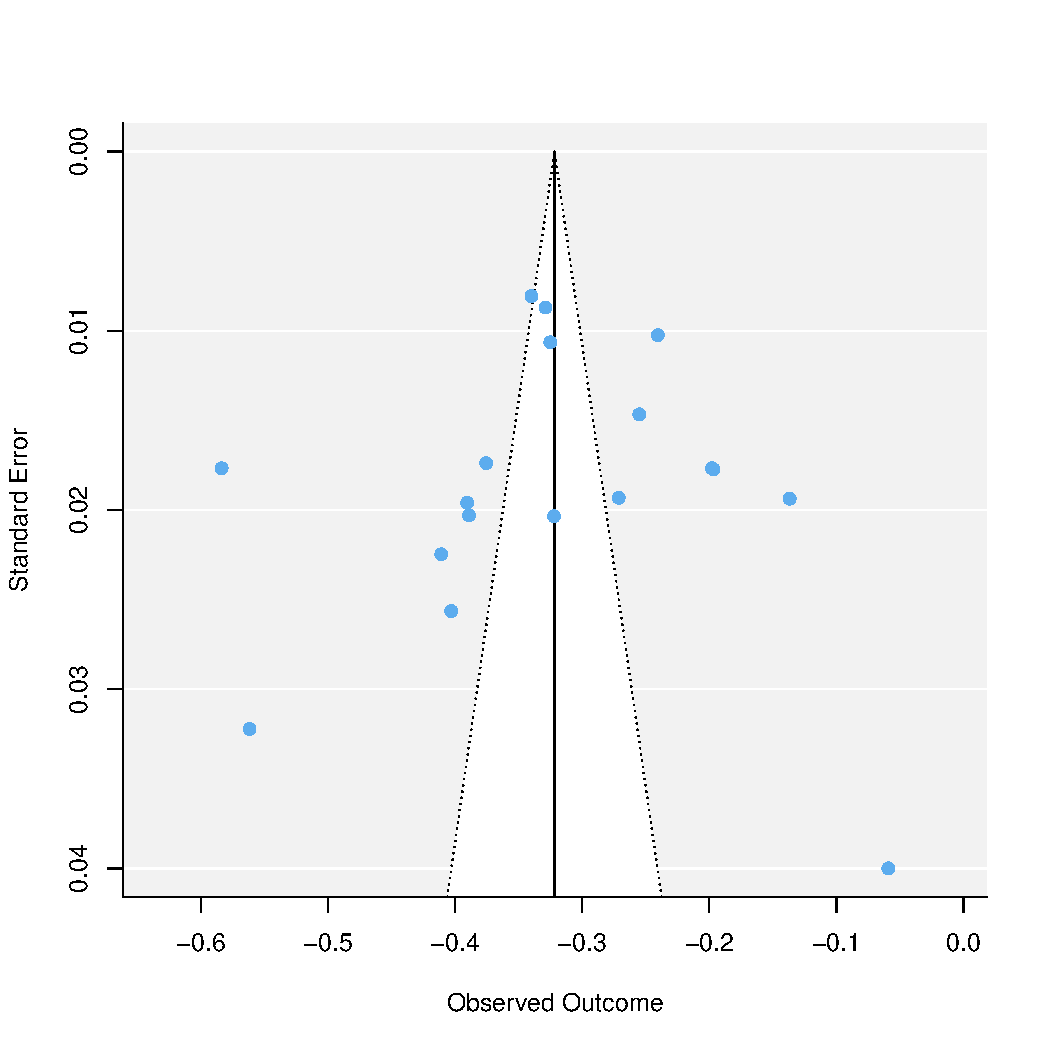
\includegraphics[scale=0.54]{../figs/funnel_re_survey.pdf}
\vspace{0.2cm}
\caption{Funnel plot: survey experiments}.
\small
\vspace{-0.3cm}
\label{fig: funnel_re_survey}
\end{centering}
\end{figure}

\begin{table}[ht] \centering 
  \caption{Regression tests for funnel plot asymmetry}
  \label{tab: funnel} 
  \small
  \vspace{0.5cm}
\begin{tabular}{@{\extracolsep{88pt}} cccccccc} 
\\[-1.8ex]\hline 
\hline \\[-1.8ex] 
 Studies included & p-value \\ 
 \hline \\[-1.8ex] 
All & 0.0016  \\
All with moderator & 0.4512  \\
Field &  0.8403  \\
Survey & 0.3159  \\
\hline \\[-1.8ex] 
\vspace{128in}
\end{tabular} 
\end{table} 
\FloatBarrier

\pagebreak
\subsection{Information quality}

\begin{figure}[!htb]
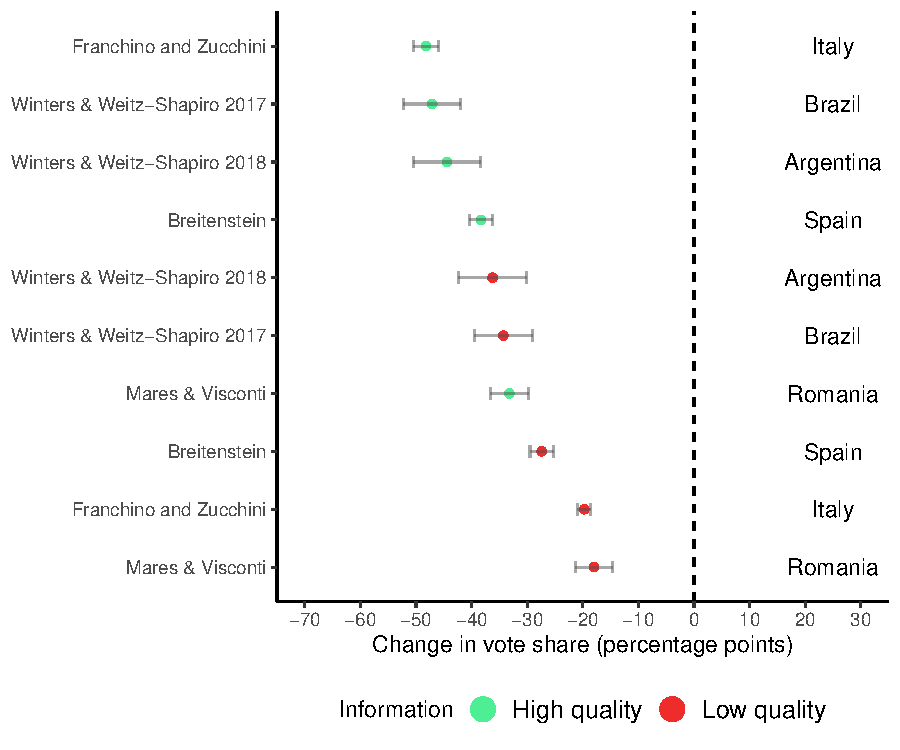
\includegraphics[scale=0.93]{../figs/quality.pdf}
\vspace{0.2cm}
\caption{Survey experiments by information quality: Average treatment effect of corruption information on vote share}.
\small
\vspace{-0.3cm}
\label{fig: quality}
\end{figure}



\end{document} 